\section{Evaluation on Synthetic Data}
\label{sec:evasim}

Evaluation on synthetic data is used to establish the benefit of POPPs' variations over the POPP in estimating the arrival rate $\lambda$ of a Poisson process. With synthetic data, sensor reliability can be controlled, and the true $\lambda$ and the true counts $c_i$ are known in advance for each sample. Based on the result that is shown in \cite{jovan18a}, we assume that the POPP outperforms the FOPP in simulated data. Hence, the FOPP is not included here for comparison.

Here, an evaluation and a comparison of the POPP models to the FOPP model are conducted with two imaginary unreliable sensors and simulated datasets. The switching filter is chosen as a filter for all POPP models for this evaluation. 

In each experiment, the sensor model (for the POPP and POPP-Beta models) and joint sensor model (for the C-POPP and POPP-Dirichlet models) were first built based on the sampled counts $c_1, \ldots, c_n$ from a Poisson process $P(c ; \lambda'=3)$ and the corresponding sensor readings $\protect\overrightarrow{s_1} \ldots \protect\overrightarrow{s_{n}}$. $n$ was set to 120 to build an erroneous (joint) sensor model. An erroneous sensor model was compensated in the case of the POPP-Dirichlet and the POPP-Beta models since a small number of samples only creates a loose Dirichlet and beta densities. Another set of counts $c_1, \ldots, c_{144}$ was sampled from the same process. These counts were then fed to simulated sensors that counted unreliably, producing sensor readings $\protect\overrightarrow{s_1} \ldots \protect\overrightarrow{s_{144}}$. A recursive update, then, took place on $P(\lambda ; \overrightarrow{s_i})$ using the switching filter for POPP, POPP-Beta, C-POPP, and POPP-Dirichlet models.

\begin{figure}[t!]
	\centering
	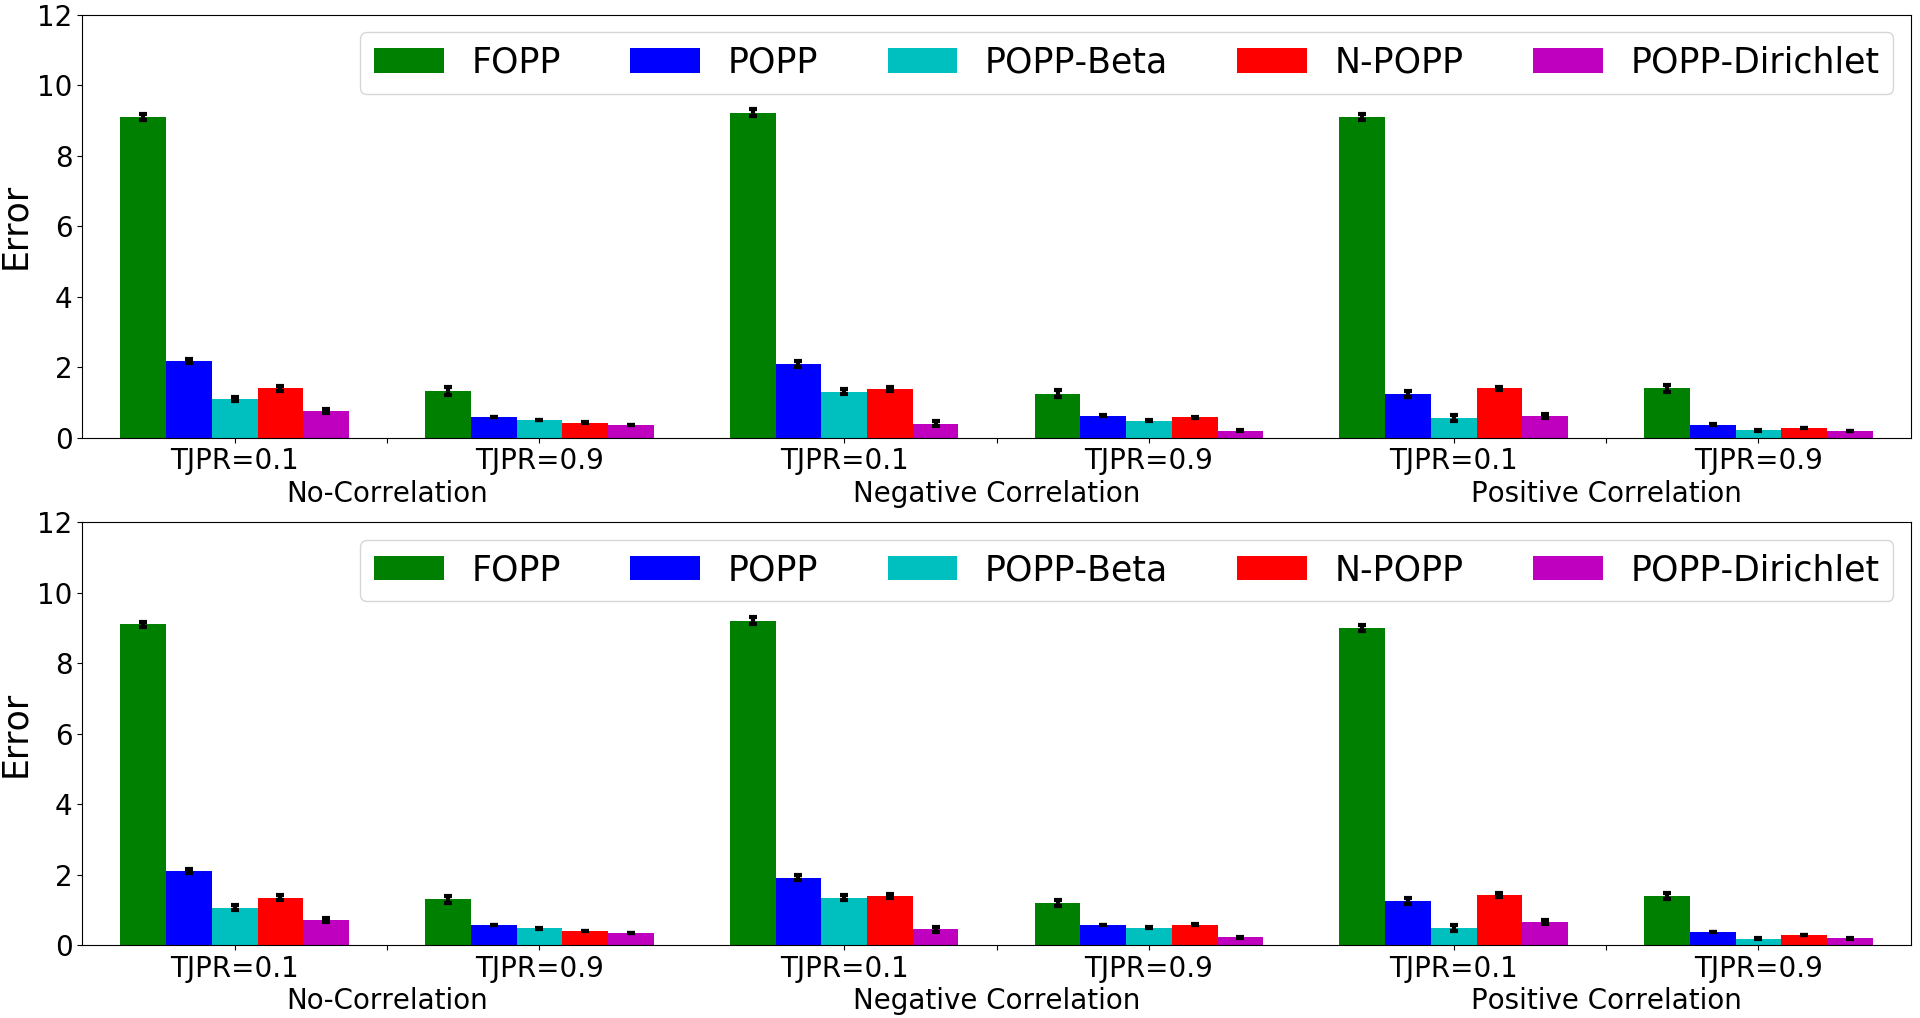
\includegraphics[width=0.5\textwidth]{./figures/tjpr_comparison_120.png}
    \caption{The RMSE of posterior estimates of $\lambda$ for the POPP-Dirichlet and other POPP models with 120 sample data used to build the (joint) sensor model with variation on $\mathcal{E^+}$. Each trial consisted of a stream of $\protect\overrightarrow{s_1} \ldots \protect\overrightarrow{s_{144}}$ samples to update $P(\lambda ; \protect\overrightarrow{s_i})$. Accuracies of MAP estimates are shown in the top panel, accuracies of expectation of the posterior in the bottom panel. Each data point is an average of 30 trials. Standard errors are shown.} 
	\label{fig:tjpr_comparison_120}
\end{figure}

\begin{figure}[t!]
	\centering
	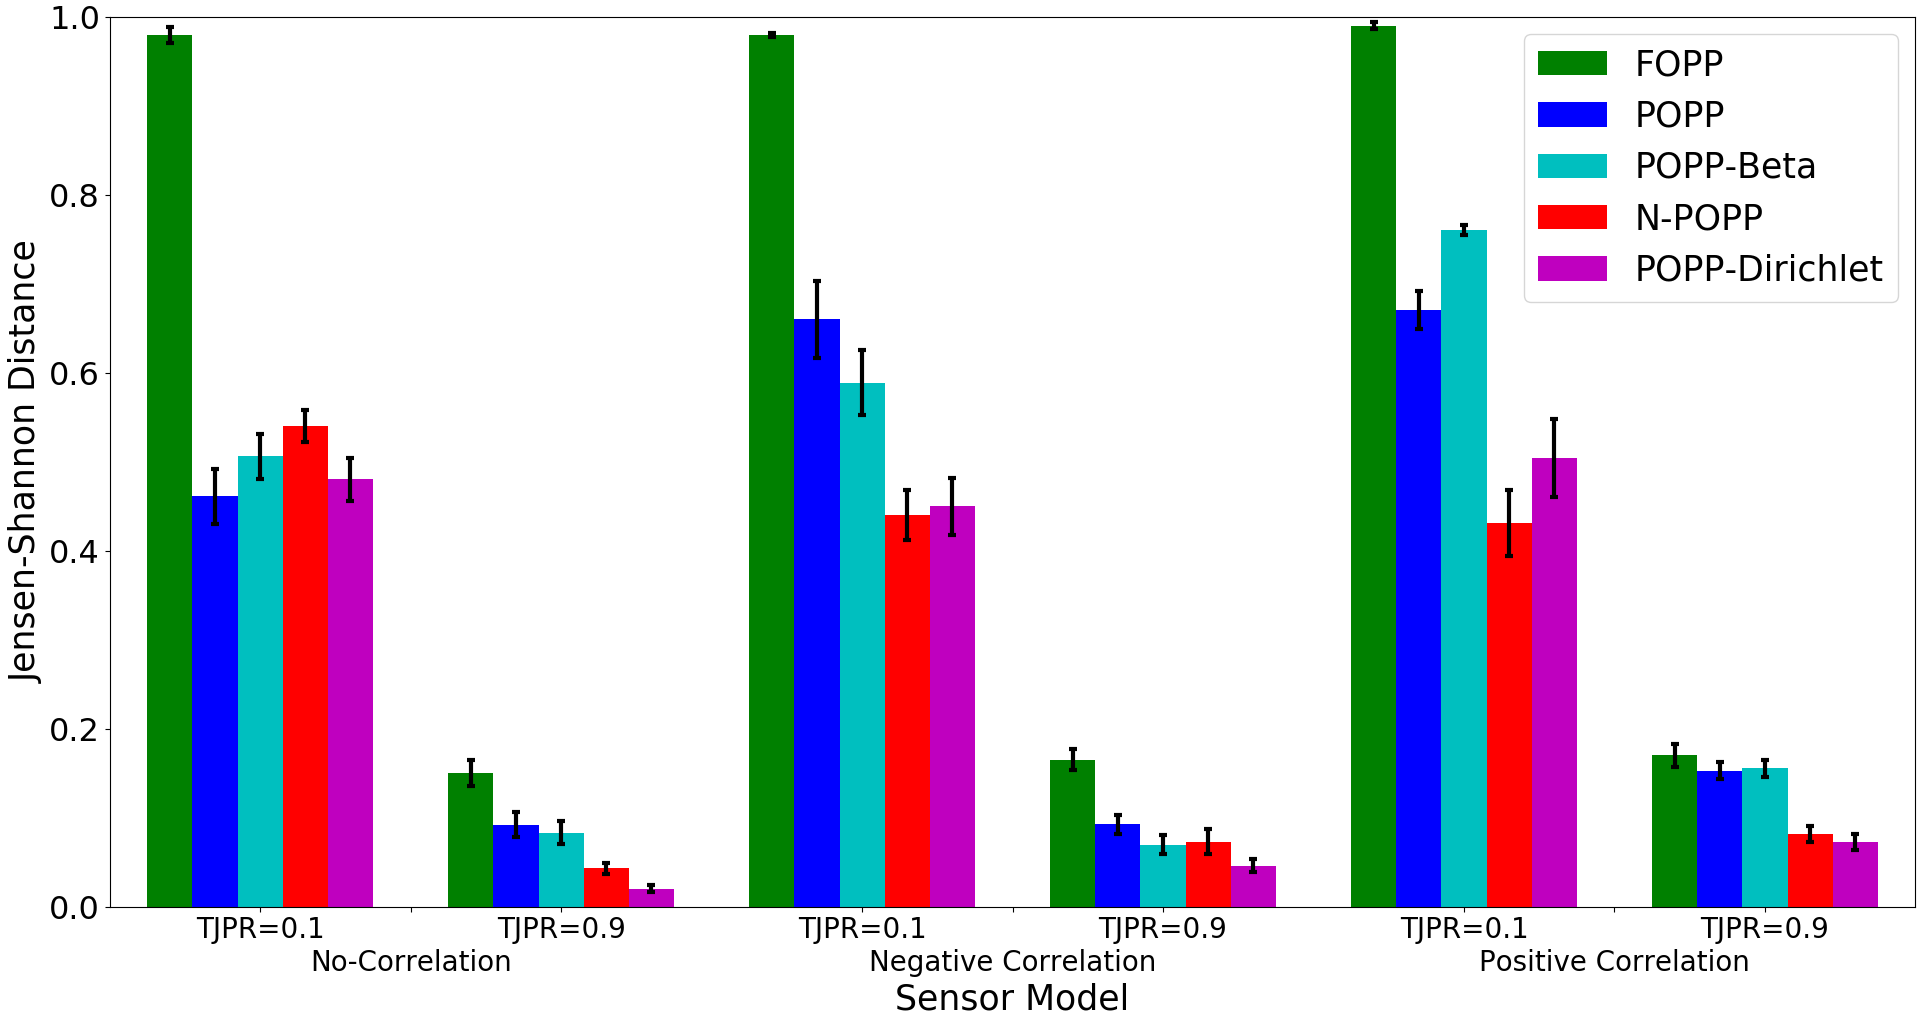
\includegraphics[width=0.5\textwidth]{./figures/tjpr_comparison_120_kl.png}
	\caption{The Jensen-Shannon distance of posterior estimates of $\lambda$ for the POPP-Dirichlet and other POPP models with 120 sample data used to build the (joint) sensor model with variation on $\mathcal{E^+}$. Each trial consisted of a stream of $\protect\overrightarrow{s_1} \ldots \protect\overrightarrow{s_{144}}$ samples to update $P_G(\lambda \mid \protect\overrightarrow{s_i})$. Each data point is an average of 30 trials. Standard errors are shown.} 
	\label{fig:tjpr_comparison_120_kl}
\end{figure}

Different correlations between two sensors were tested: positive correlation, negative correlation, and no correlation. These correlations are aimed to show the benefit of the C-POPP and POPP-Dirichlet models over the POPP and the POPP-Beta models. One should note that under the POPP and POPP-Beta models, sensors are assumed to be uncorrelated. For each correlation type, a further variation to different levels of sensor unreliability was considered. The true joint positive rate $\mathcal{E^+}$ (TJPR) and the true joint negative rate $\mathcal{E^-}$ (TJNR) were set as basis for varying sensor unreliability. For example, having TJPR configured with $P_{jnt}(d_{1k}=1, d_{2k}=1 ; e_k=1) = 0.1, P_{jnt}(d_{1k}=0, d_{2k}=0 ; e_k=1) = 0.9$ means that the true positive rate (TPR) for each sensor $j$ is $\textrm{\textit{tpr}}_j = P_j(d_k = 1; e_k=1) = 0.1$.

First, two variations were made to the true joint positive rate $\mathcal{E^+}$ (TJPR), while fixing the true joint negative rate $\mathcal{E^-}$ (TJNR) on each type of correlation. This includes:
\begin{itemize}
    \item $P_{jnt}(d_{1k}=1, d_{2k}=1 ; e_k=1) = 0.1, P_{jnt}(d_{1k}=0, d_{2k}=0 ; e_k=1) = 0.9$ ($\mathcal{E^+}$ with low positive correlation);
    \item $P_{jnt}(d_{1k}=1, d_{2k}=1 ; e_k=1) = 0.9, P_{jnt}(d_{1k}=0, d_{2k}=0 ; e_k=1) = 0.1$ ($\mathcal{E^+}$ with high positive correlation);
    \item $P_{jnt}(d_{1k}=1, d_{2k}=0 ; e_k=1) = 0.05, P_{jnt}(d_{1k}=0, d_{2k}=1 ; e_k=1) = 0.05, P_{jnt}(d_{1k}=0, d_{2k}=0 ; e_k=1) = 0.9$ ($\mathcal{E^+}$ with low negative correlation);
    \item $P_{jnt}(d_{1k}=1, d_{2k}=0 ; e_k=1) = 0.45, P_{jnt}(d_{1k}=0, d_{2k}=1 ; e_k=1) = 0.45, P_{jnt}(d_{1k}=0, d_{2k}=0 ; e_k=1) = 0.1$ ($\mathcal{E^+}$ with high negative correlation);
    \item $P_{jnt}(d_{1k}=1, d_{2k}=0 ; e_k=1) = 0.033, P_{jnt}(d_{1k}=0, d_{2k}=1 ; e_k=1) = 0.033, P_{jnt}(d_{1k}=1, d_{2k}=1 ; e_k=1) = 0.033, P_{jnt}(d_{1k}=0, d_{2k}=0 ; e_k=1) = 0.901$ ($\mathcal{E^+}$ with no correlation -- Similar to a sensor model with TPR = 0.066);
    \item $P_{jnt}(d_{1k}=1, d_{2k}=0 ; e_k=1) = 0.3, P_{jnt}(d_{1k}=0, d_{2k}=1 ; e_k=1) = 0.3, P_{jnt}(d_{1k}=1, d_{2k}=1 ; e_k=1) = 0.3, P_{jnt}(d_{1k}=0, d_{2k}=0 ; e_k=1) = 0.1$ ($\mathcal{E^+}$ with no correlation -- Similar to a sensor model with TPR = 0.6).
\end{itemize}

Second, two variations to the true joint negative rate $\mathcal{E^-}$ (TJNR), while fixing the true joint positive rate $\mathcal{E^+}$ (TJPR) on each type of correlation. This includes: 
\begin{itemize}
	\item $P_{jnt}(d_{1k}=1, d_{2k}=1 ; e_k=0) = 0.1, P_{jnt}(d_{1k}=0, d_{2k}=0 ; e_k=0) = 0.9$ ($\mathcal{E^-}$ with low positive correlation);
	\item $P_{jnt}(d_{1k}=1, d_{2k}=1 ; e_k=0) = 0.9, P_{jnt}(d_{1k}=0, d_{2k}=0 ; e_k=0) = 0.1$ ($\mathcal{E^-}$ with high positive correlation);
	\item $P_{jnt}(d_{1k}=1, d_{2k}=0 ; e_k=0) = 0.05, P_{jnt}(d_{1k}=0, d_{2k}=1 ; e_k=0) = 0.05, P_{jnt}(d_{1k}=0, d_{2k}=0 ; e_k=0) = 0.9$ ($\mathcal{E^-}$ with low negative correlation);
	\item $P_{jnt}(d_{1k}=1, d_{2k}=0 ; e_k=0) = 0.45, P_{jnt}(d_{1k}=0, d_{2k}=1 ; e_k=0) = 0.45, P_{jnt}(d_{1k}=0, d_{2k}=0 ; e_k=0) = 0.1$ ($\mathcal{E^-}$ with high negative correlation);
	\item $P_{jnt}(d_{1k}=1, d_{2k}=0 ; e_k=0) = 0.033, P_{jnt}(d_{1k}=0, d_{2k}=1 ; e_k=0) = 0.033, P_{jnt}(d_{1k}=1, d_{2k}=1 ; e_k=0) = 0.033, P_{jnt}(d_{1k}=0, d_{2k}=0 ; e_k=1) = 0.901$ ($\mathcal{E^-}$ with no correlation -- Similar to a sensor model with low TNR);
	\item $P_{jnt}(d_{1k}=1, d_{2k}=0 ; e_k=0) = 0.3, P_{jnt}(d_{1k}=0, d_{2k}=1 ; e_k=0) = 0.3, P_{jnt}(d_{1k}=1, d_{2k}=1 ; e_k=0) = 0.3, P_{jnt}(d_{1k}=0, d_{2k}=0 ; e_k=1) = 0.1$ ($\mathcal{E^-}$ with no correlation -- Similar to a sensor model with moderate TNR).
\end{itemize}

The performance of all POPP models were assessed by comparing how accurate each model is in estimating the true $\lambda'$. Two options were used to do this: (1) a distance metric method using the RMSE of the expectation (mean) and the MAP hypothesis (mode) of each model posterior distribution over $\lambda$ to the true $\lambda'$ and (2) a free-distance metric method using the Jensen-Shannon distance between the posterior distribution $P(\lambda ; \overrightarrow{s_i})$ and the distribution of the true $\lambda'$. 

\begin{figure}[t!]
	\centering
	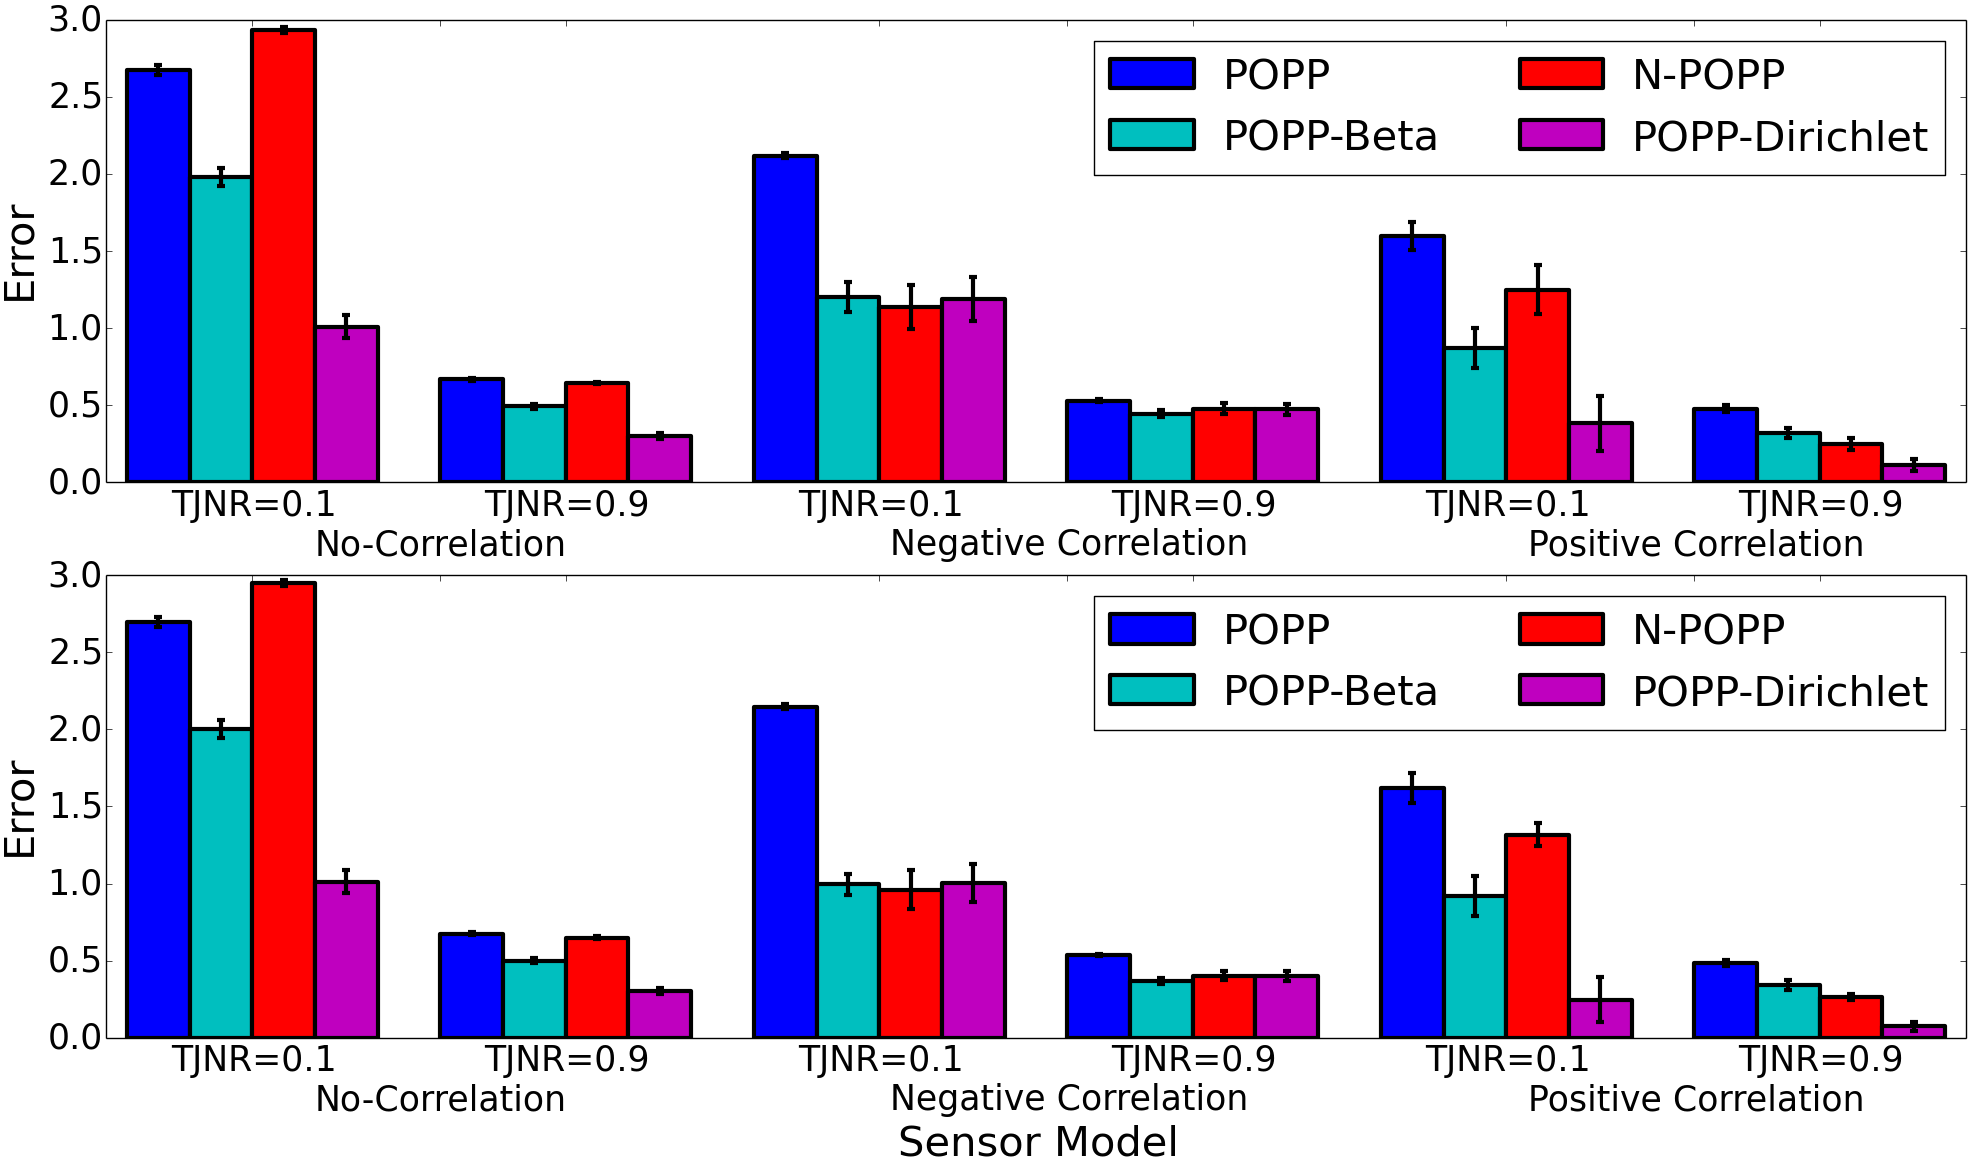
\includegraphics[width=0.5\textwidth]{./figures/tjnr_comparison_120.png}
    \caption{The RMSE of posterior estimates of $\lambda$ for the POPP-Dirichlet and other POPP models with 120 sample data used to build the (joint) sensor model with variation in $\mathcal{E^-}$. Each trial consisted of a stream of $\protect\overrightarrow{s_1} \ldots \protect\overrightarrow{s_{144}}$ samples to update $P(\lambda ; \protect\overrightarrow{s_i})$. Accuracies of MAP estimates are  in the top panel, accuracies of the expectation of the posterior in the bottom panel. Each data point is an average of 30 trials. Standard errors are shown.} 
	\label{fig:tjnr_comparison_120}
\end{figure}

\begin{figure}[t!]
	\centering
	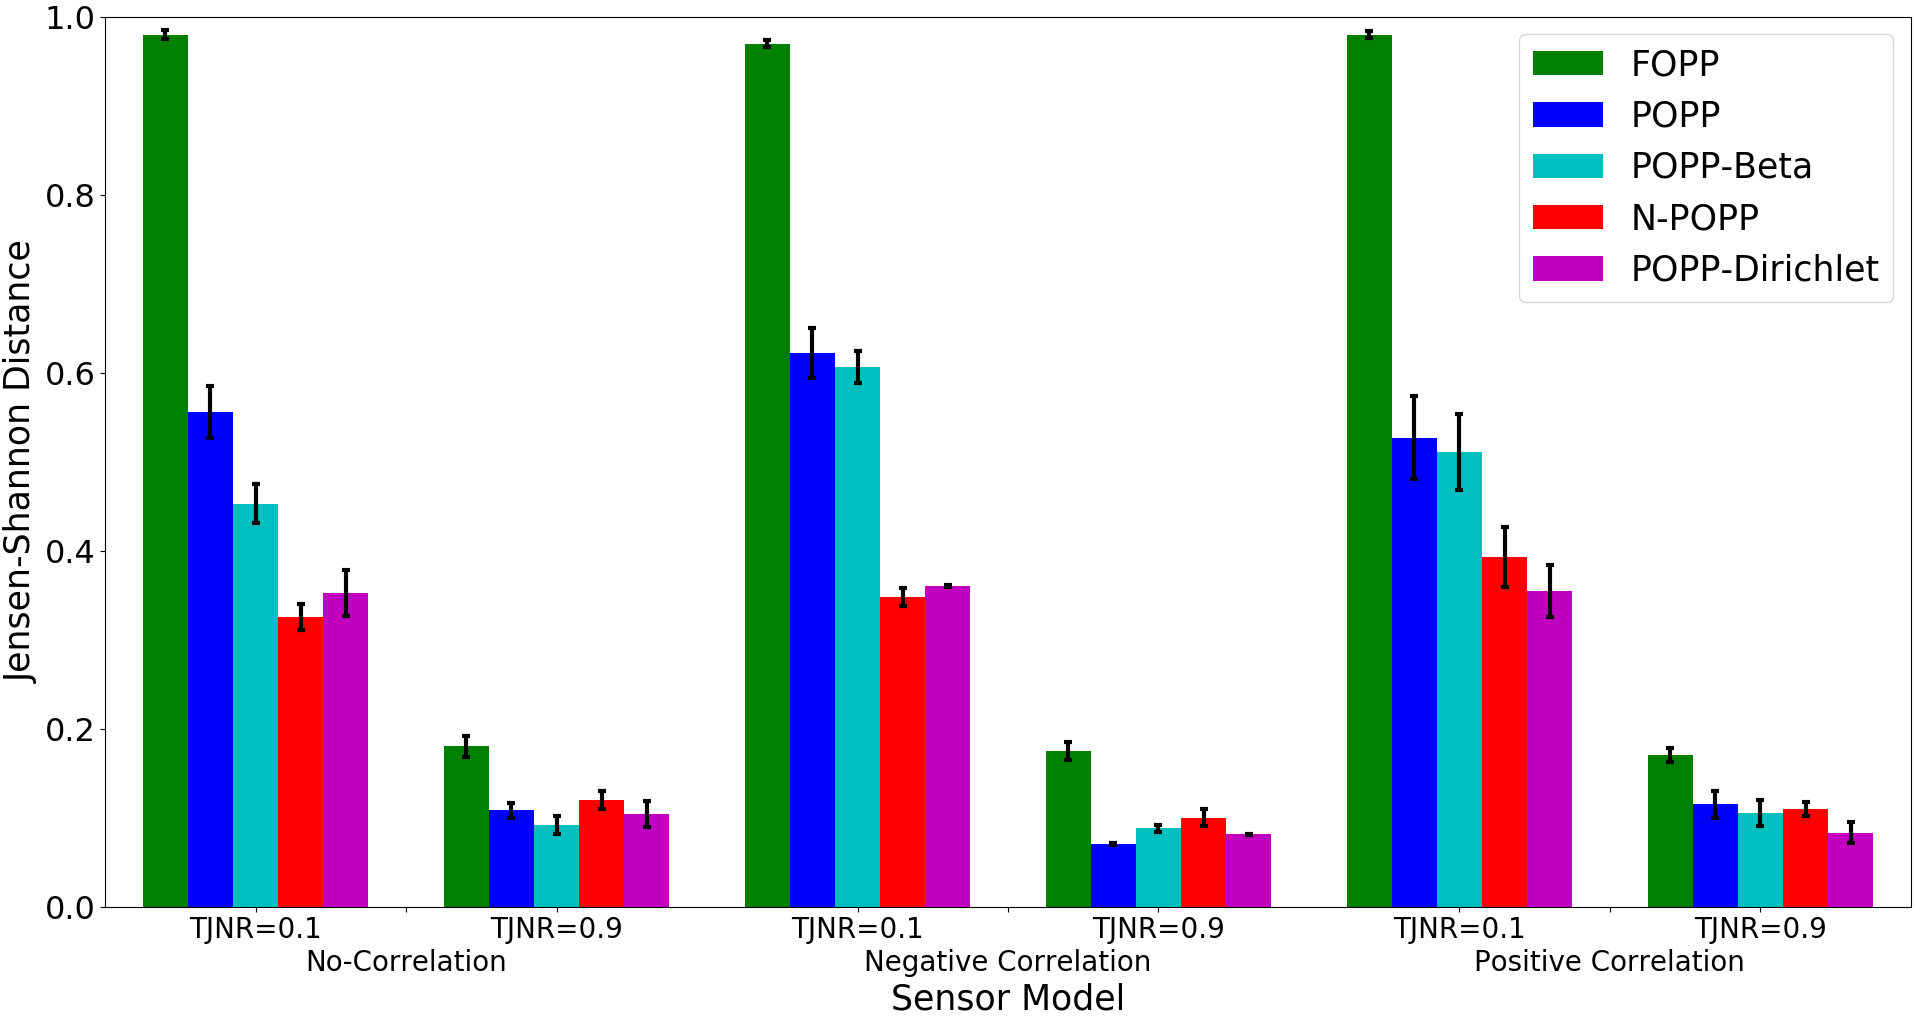
\includegraphics[width=0.5\textwidth]{./figures/tjnr_comparison_120_kl.png}
	\caption{The Jensen-Shannon distance of posterior estimates of $\lambda$ for the POPP-Dirichlet and other POPP models with 120 sample data used to build the (joint) sensor model with variation on $\mathcal{E^-}$. Each trial consisted of a stream of $\protect\overrightarrow{s_1} \ldots \protect\overrightarrow{s_{144}}$ samples to update $P_G(\lambda \mid \protect\overrightarrow{s_i})$. Each data point is an average of 30 trials. Standard errors are shown.} 
	\label{fig:tjnr_comparison_120_kl}
\end{figure}

Figure \ref{fig:tjpr_comparison_120} and \ref{fig:tjpr_comparison_120_kl} show the accuracy of all POPP models on the variation of true joint positive rate, whereas figure \ref{fig:tjnr_comparison_120} and \ref{fig:tjnr_comparison_120_kl} show the accuracy on the variation of the true joint negative rate. From these figures, the POPP-Beta and POPP-Dirichlet show a better accuracy than the POPP and the C-POPP. The C-POPP and the POPP-Dirichlet which utilize correlation among sensors to estimate the arrival rate $\lambda'$ tend to be more accurate than the standard POPP and POPP-Beta.
In general, the POPP-Dirichlet tends to be more accurate than any other POPP model thanks to its ability to model correlation among sensors and to model how confident it is with its sensor model.
